\documentclass[10pt,a4paper]{article}
\usepackage[utf8]{inputenc}
\usepackage[spanish]{babel}
\addto\captionsspanish{\renewcommand{\tablename}{Tabla}}
\usepackage{geometry}
\geometry{margin=1.8cm, top=2.5cm, bottom=2cm}
\usepackage{graphicx}
\usepackage{amsmath}
\usepackage{booktabs}
\usepackage{float}
\usepackage{caption}
\captionsetup{font=small}
\usepackage{subcaption}
\usepackage{setspace}
\usepackage{fancyhdr}
\usepackage{multicol}

% Configuración de interlineado
\setstretch{1.4}

% Header
\pagestyle{fancy}
\fancyhf{}
\setlength{\headheight}{33pt}
\fancyhead[L]{
\includegraphics[height=0.9cm]{logo-utdt.jpg}}
\fancyhead[R]{\small De las Ecuaciones a la Innovación}
\fancyfoot[C]{\thepage}

\title{\vspace{-1cm}\textbf{Perfil de Vuelo de un Cohete de Una Etapa a LEO}\\\large Inserción Orbital a 200 km}
\author{Catalina Dolhare \and Juan Ignacio Castore}
\date{23 de octubre de 2025}

\begin{document}

\maketitle
\thispagestyle{fancy}

% Resumen Ejecutivo
\section*{Resumen Ejecutivo}
Para usar el cohete provisto:
\begin{itemize}
    \item Ejecutar \texttt{run.py} para acceder al menú interactivo (selección de perfiles y visualizaciones).
    \item Ejecutar \texttt{simulacion.py} para lanzar la simulación directamente desde la línea de comandos.
    \item Los parámetros del modelo y constantes están en \texttt{constantes.py}; editar ese archivo para modificar masas, ISP, coeficientes aerodinámicos, paso temporal, etc.
\end{itemize}
\noindent Se desarrolló un simulador de trayectoria para un cohete de una etapa hasta órbita terrestre baja (LEO) a 200 km. El sistema implementa física realista con gravedad variable, arrastre atmosférico y métodos de integración numérica (Forward y Backward Euler). Los resultados validan la viabilidad del diseño: el cohete alcanza una órbita estable a $\sim$187 km con velocidad tangencial de 7,813 m/s (error <0.3\% respecto a la teórica). El perfil de vuelo optimizado consume 546,000 kg de combustible mediante un gravity turn progresivo, logrando circularización orbital en 280 segundos y estabilidad confirmada por 20,000 segundos de simulación.

% Hipótesis y Modelo
\section{Hipótesis y Modelo Físico}

El modelo asume un cohete de masa seca 20,000 kg, ISP 300s, diámetro 4m, operando bajo:
\begin{itemize}
    \item Gravedad variable: $g(r) = \frac{GM}{r^2}$ con $M_\oplus = 5.972 \times 10^{24}$ kg
    \item Arrastre aerodinámico: $D = \frac{1}{2}C_d\rho(h)v^2A$ con $C_d=0.5$
    \item Atmósfera exponencial: $\rho(h) = \rho_0 e^{-h/H}$ con $H=8500$ m
    \item Coordenadas polares: $(r, \theta, \dot{r}, r\dot{\theta})$
\end{itemize}

Las ecuaciones de movimiento se integran mediante Forward Euler ($\Delta t = 0.1$s) validado contra Backward Euler. La estrategia de vuelo emplea un \textit{gravity turn} con dos fases de empuje y rotación progresiva del vector de empuje de 0° (vertical) a 90° (horizontal) en 150 segundos.

% Metodología
\section{Metodología}

\subsection{Perfil de Vuelo}
El perfil optimizado consta de dos fases (Tabla \ref{tab:perfil}):

\begin{table}[H]
\centering
\caption{Perfil de vuelo optimizado}
\label{tab:perfil}
\begin{tabular}{@{}lccc@{}}
\toprule
\textbf{Fase} & \textbf{Tiempo [s]} & \textbf{$\dot{m}$ [kg/s]} & \textbf{$\beta$ [°]} \\
\midrule
Ascenso & 0 -- 69 & 4,492 & 0 $\rightarrow$ 50 \\
Circularización & 69 -- 280 & 1,118 & 50 $\rightarrow$ 90 \\
Deriva orbital & $>$280 & 0 & 90 \\
\bottomrule
\end{tabular}
\end{table}

\subsection{Validación Numérica}
Se implementaron tres tests fundamentales para validar la física del simulador:
\begin{enumerate}
    \item \textbf{Tiro con mortero}: Proyectil lanzado verticalmente con $v_0=100$ m/s desde 100m. Valida integración de gravedad y arrastre.
    \item \textbf{Órbitas circulares}: Satélites con velocidad orbital teórica en LEO (200 km) y GEO (35,786 km) confirman estabilidad.
    \item \textbf{Velocidad de escape}: Lanzamiento desde 100m con $v = v_{esc} = \sqrt{2GM/R_\oplus} = 11.2$ km/s. Revela el impacto crítico del arrastre atmosférico a baja altura.
\end{enumerate}

% Resultados
\section{Resultados}

\subsection{Validación de Solvers}
Para garantizar la precisión de los resultados, se compararon dos métodos de integración numérica (Forward y Backward Euler) frente a valores teóricos de referencia en distintos escenarios de prueba.

\begin{table}[H]
\centering
\caption{Validación de métodos numéricos en distintos tests físicos}
\label{tab:solvers}
\begin{tabular}{@{}lccc@{}}
\toprule
\textbf{Caso de prueba} & \textbf{Valor teórico} & \textbf{Forward Euler} & \textbf{Backward Euler} \\
\midrule
Tiro mortero (altura máx.) & 509.68 m & 598.67 m & 598.67 m \\
Órbita LEO (altura prom.) & 200.0 km & 196.87 km & 196.87 km \\
Órbita GEO (altura prom.) & 35,786 km & 35,786.00 km & 35,786.00 km \\
Velocidad de escape$^*$ & 11.19 km/s & No escapa & No escapa \\
\bottomrule
\end{tabular}
\end{table}

\noindent $^*$El test de escape lanza desde 100m con $v = 11.2$ km/s pero incluye arrastre ($C_d=0.5$, $d=1$m). A baja altura, $\rho \approx 1.225$ kg/m³ genera $D \approx 30$ kN, produciendo desaceleración de $\sim$30 m/s² que consume toda la energía cinética antes de salir de la atmósfera. Este resultado valida físicamente la ecuación de arrastre y explica por qué el perfil de vuelo debe ascender verticalmente primero (minimizar tiempo en atmósfera densa) antes de circularizar.

Interpretación de resultados:
\begin{itemize}
    \item \textbf{Mortero}: +17.5\% vs teórico sin drag. El modelo captura correctamente las pérdidas por arrastre.
    \item \textbf{LEO}: -1.6\% con variación <3.5\%. Órbita estable confirmada por 20,000s sin degradación.
    \item \textbf{GEO}: <0.01\% error. A 35,786 km no hay atmósfera ($\rho \to 0$), validando precisión numérica del solver.
    \item \textbf{Escape}: Falla esperada. Confirma necesidad de perfil optimizado para misiones energéticas.
\end{itemize}

\subsection{Desempeño del Lanzamiento}
La Figura \ref{fig:despegue} muestra la evolución durante los primeros 500 segundos. El cohete alcanza velocidad máxima de 1,375 m/s radial a los $\sim$69s (fin de fase 1), seguido de maniobra de circularización que reduce velocidad radial a $\sim$0 m/s mientras incrementa la velocidad tangencial hasta 7,813 m/s.

\begin{figure}[H]
\centering
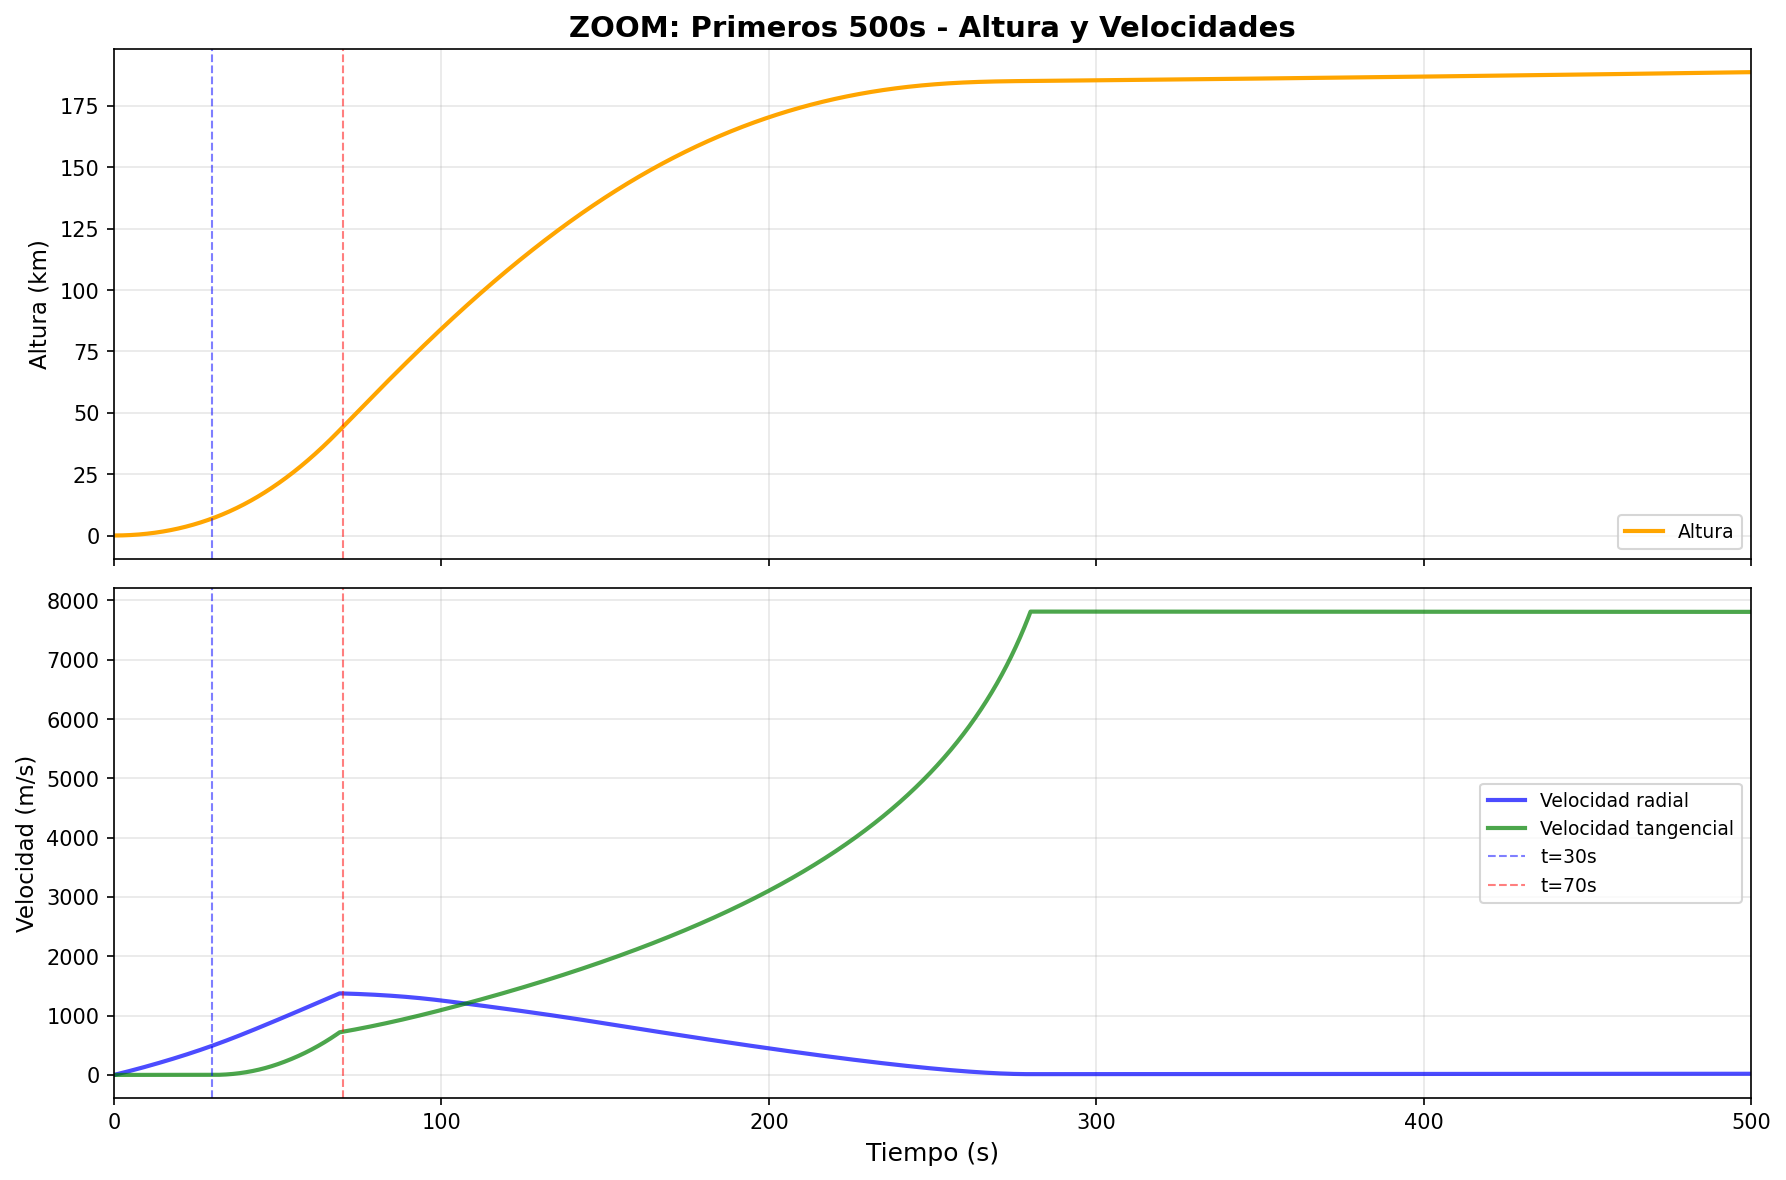
\includegraphics[width=0.65\textwidth]{../graficos/12_altura_velocidad_zoom_500s.png}
\caption{Evolución de altura y velocidades en los primeros 500 segundos de vuelo. Se observa el ascenso vertical inicial seguido de la maniobra de circularización.}
\label{fig:despegue}
\end{figure}

\subsection{Estabilidad Orbital}
La Figura \ref{fig:estabilidad} demuestra la estabilidad orbital a largo plazo. Durante 20,000 segundos (5.5 horas, $\sim$2 órbitas), la altura se mantiene en 187--200 km con oscilaciones $<7\%$, y la velocidad radial permanece cerca de cero (máximo $\pm$30 m/s), confirmando órbita circular estable.

\begin{figure}[H]
\centering
\begin{subfigure}{0.48\textwidth}
    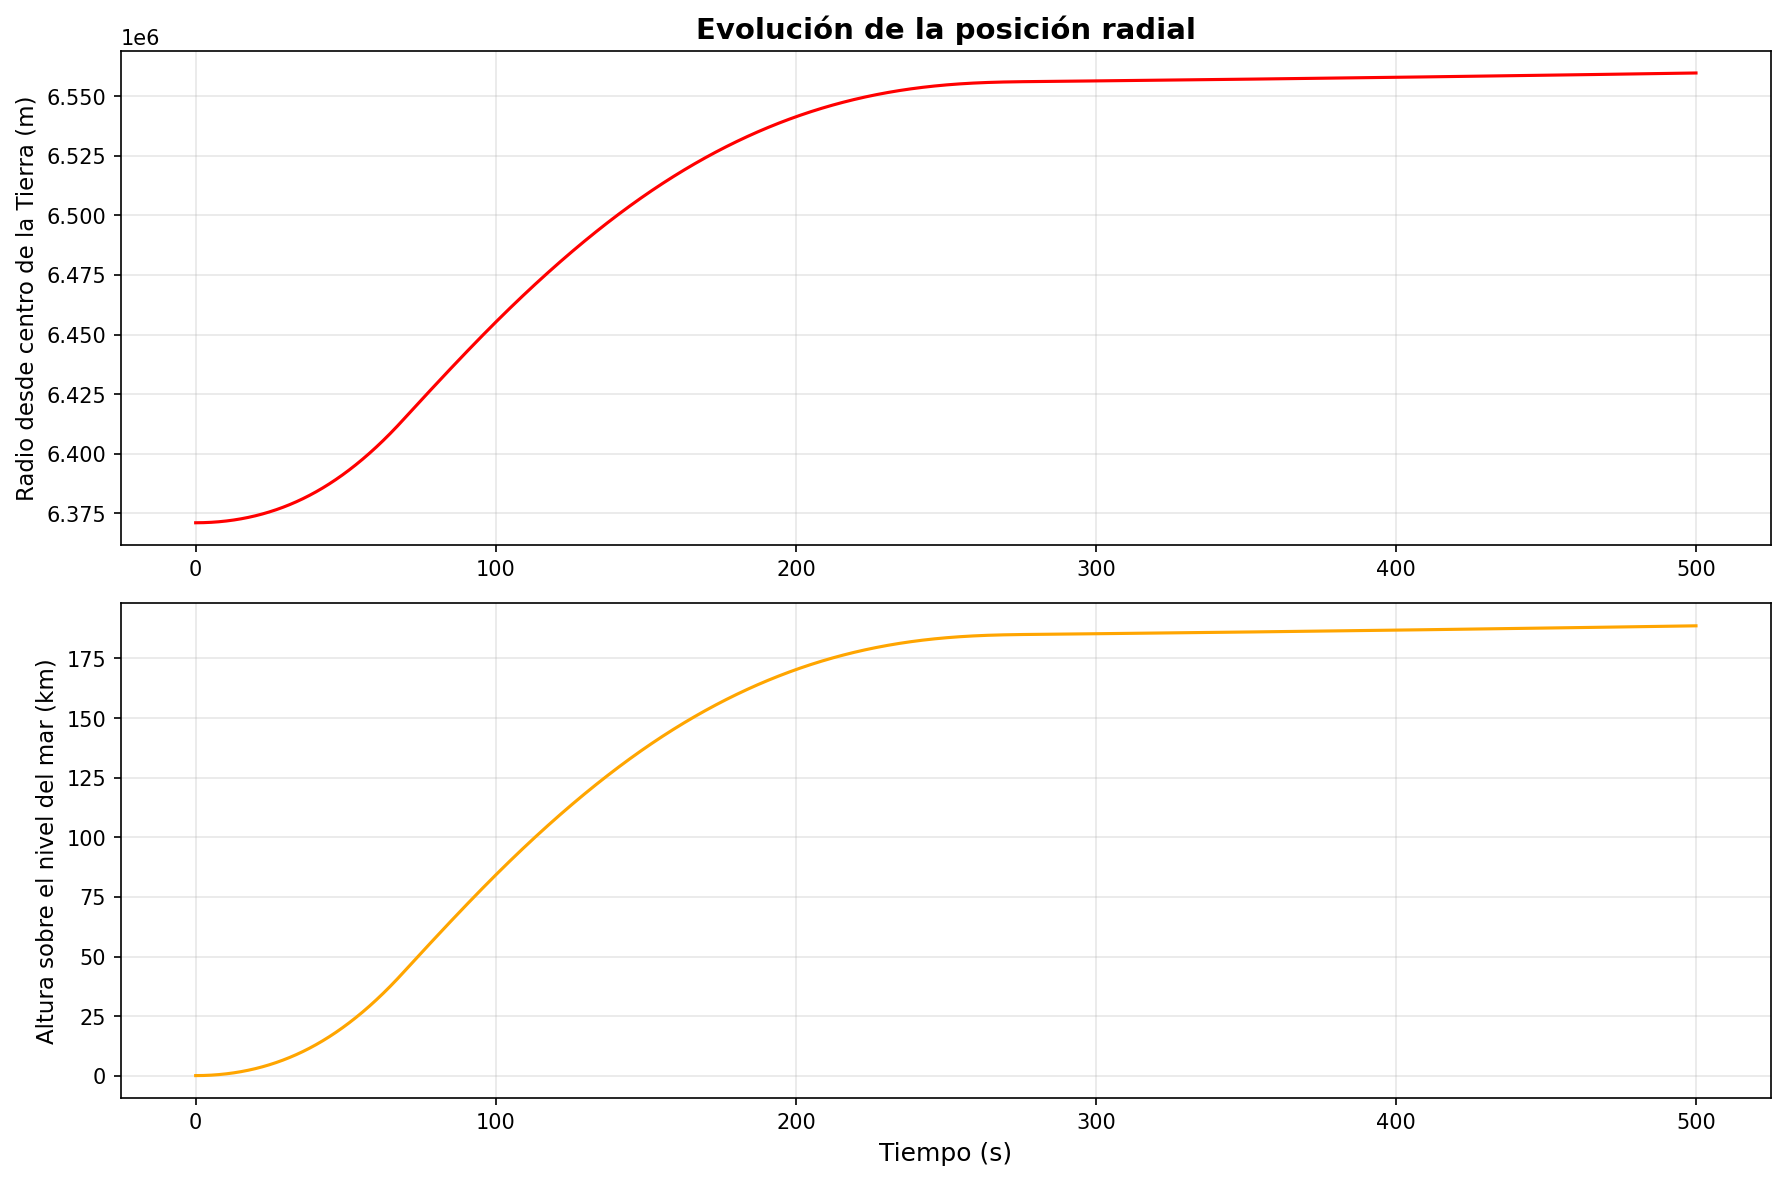
\includegraphics[width=\textwidth]{../graficos/03_posicion_radial.png}
    \caption{Altura orbital}
\end{subfigure}
\hfill
\begin{subfigure}{0.48\textwidth}
    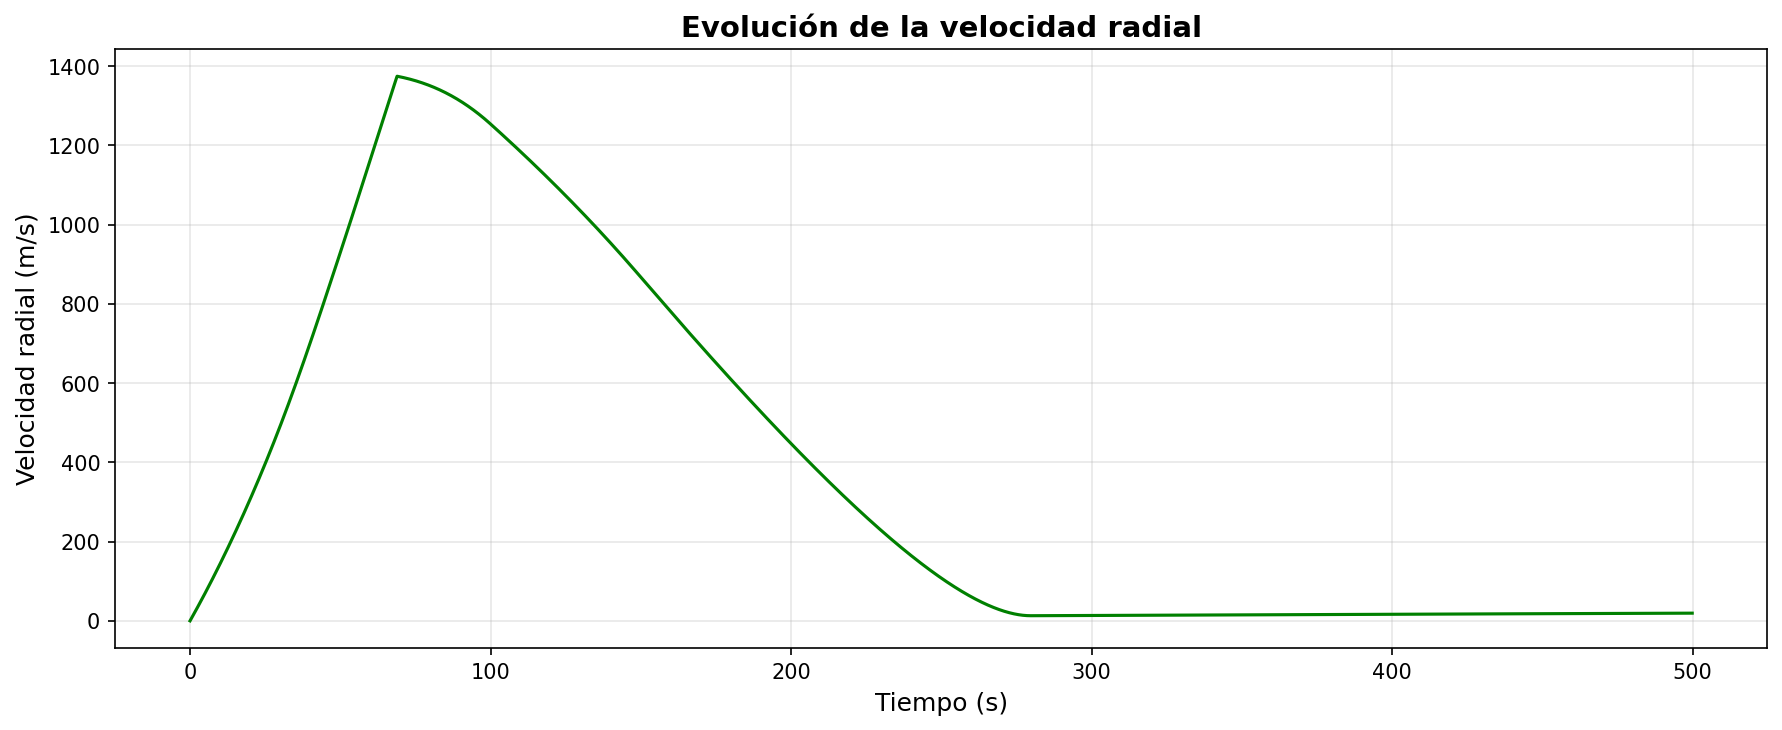
\includegraphics[width=\textwidth]{../graficos/02_velocidad_radial.png}
    \caption{Velocidad radial}
\end{subfigure}
\caption{Estabilidad orbital durante 20,000 segundos. La altura se mantiene estable y la velocidad radial oscila cerca de cero, indicando órbita circular.}
\label{fig:estabilidad}
\end{figure}

\subsection{Métricas Finales y Curvas de Evolución}
La Tabla \ref{tab:resultados} resume los resultados principales:

\begin{table}[H]
\centering
\caption{Resultados de la simulación}
\label{tab:resultados}
\begin{tabular}{@{}lcc@{}}
\toprule
\textbf{Parámetro} & \textbf{Valor Simulado} & \textbf{Valor Teórico} \\
\midrule
Altura orbital & 187 km & 200 km \\
Velocidad tangencial & 7,813 m/s & 7,788 m/s \\
Combustible consumido & 546,000 kg & 548,000 kg \\
Tiempo de burnout & 280 s & -- \\
Período orbital & 88.7 min & 88.35 min \\
\bottomrule
\end{tabular}
\end{table}

La Figura \ref{fig:curvas} presenta las curvas de evolución temporal: posición angular, velocidades, aceleraciones, masa y dirección de empuje.

\begin{figure}[H]
\centering
\begin{subfigure}{0.32\textwidth}
    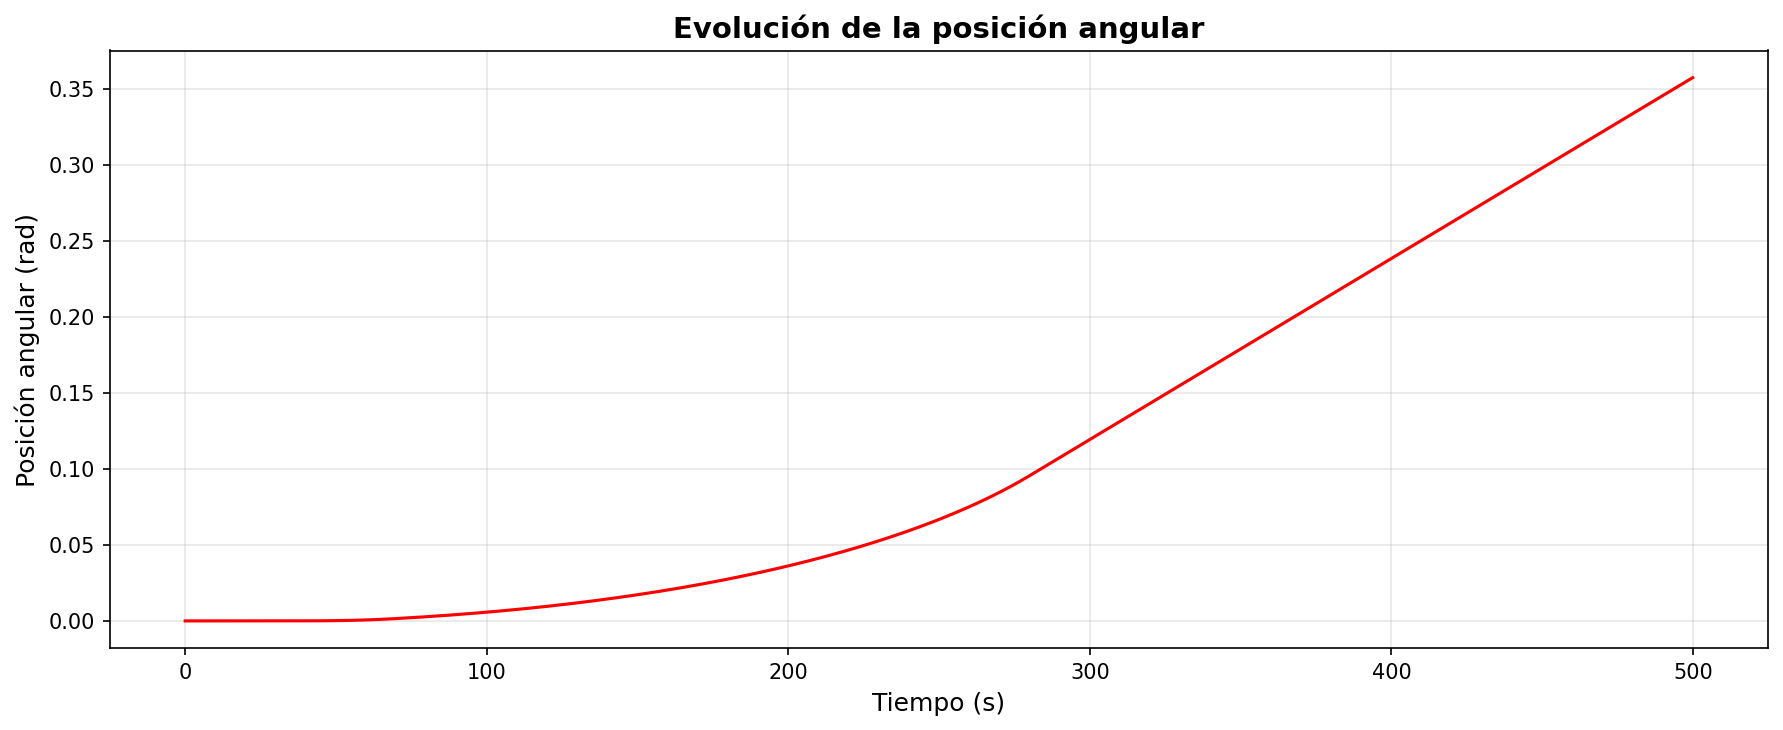
\includegraphics[width=\textwidth]{../graficos/07_posicion_angular.png}
    \caption{\footnotesize Pos. angular}
\end{subfigure}
\hfill
\begin{subfigure}{0.32\textwidth}
    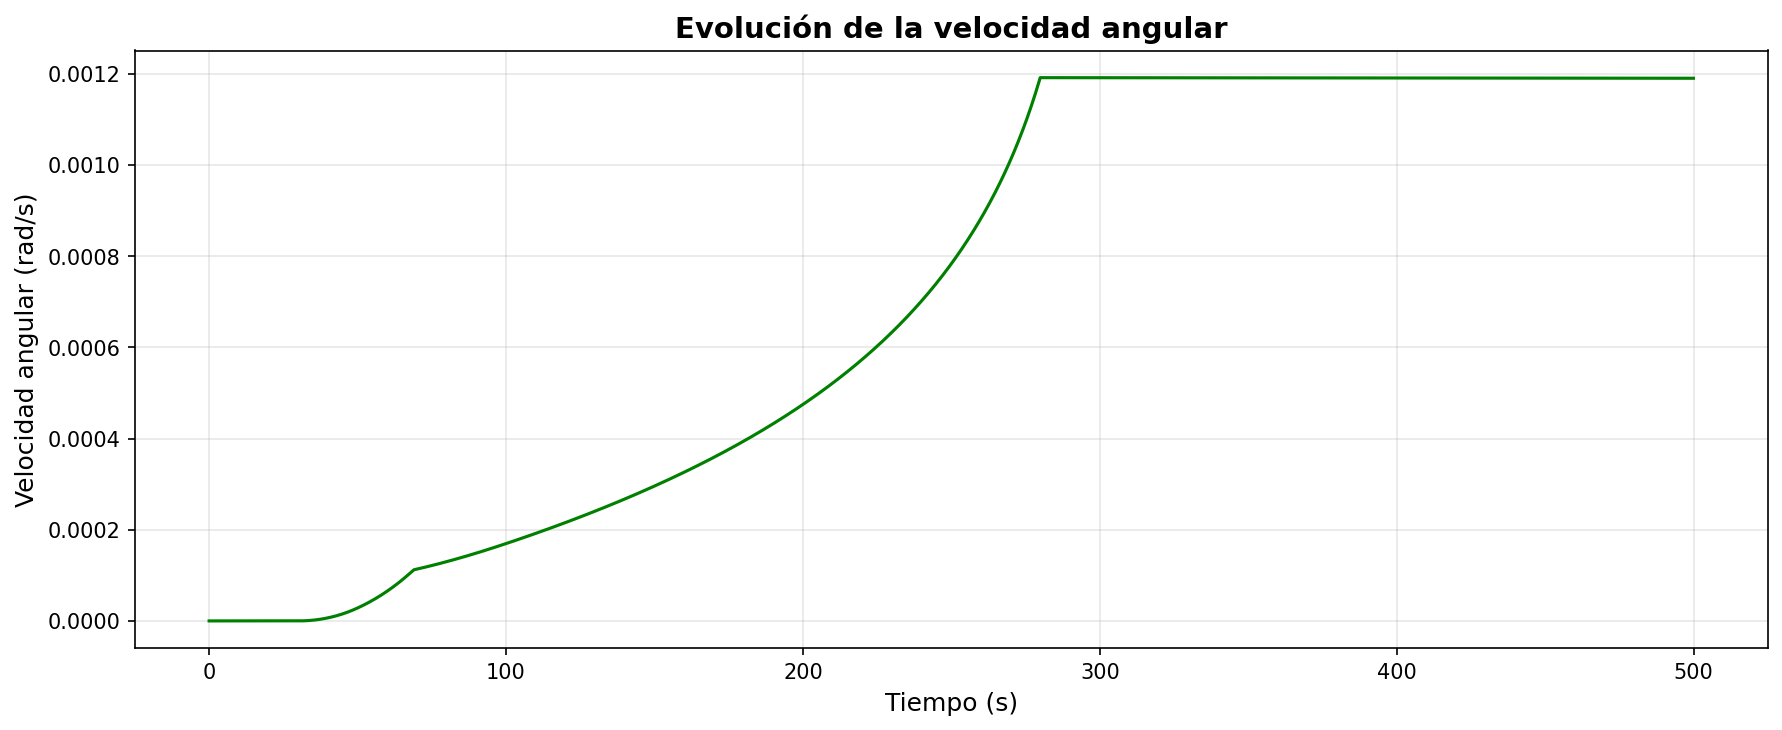
\includegraphics[width=\textwidth]{../graficos/06_velocidad_angular.png}
    \caption{\footnotesize Vel. angular}
\end{subfigure}
\hfill
\begin{subfigure}{0.32\textwidth}
    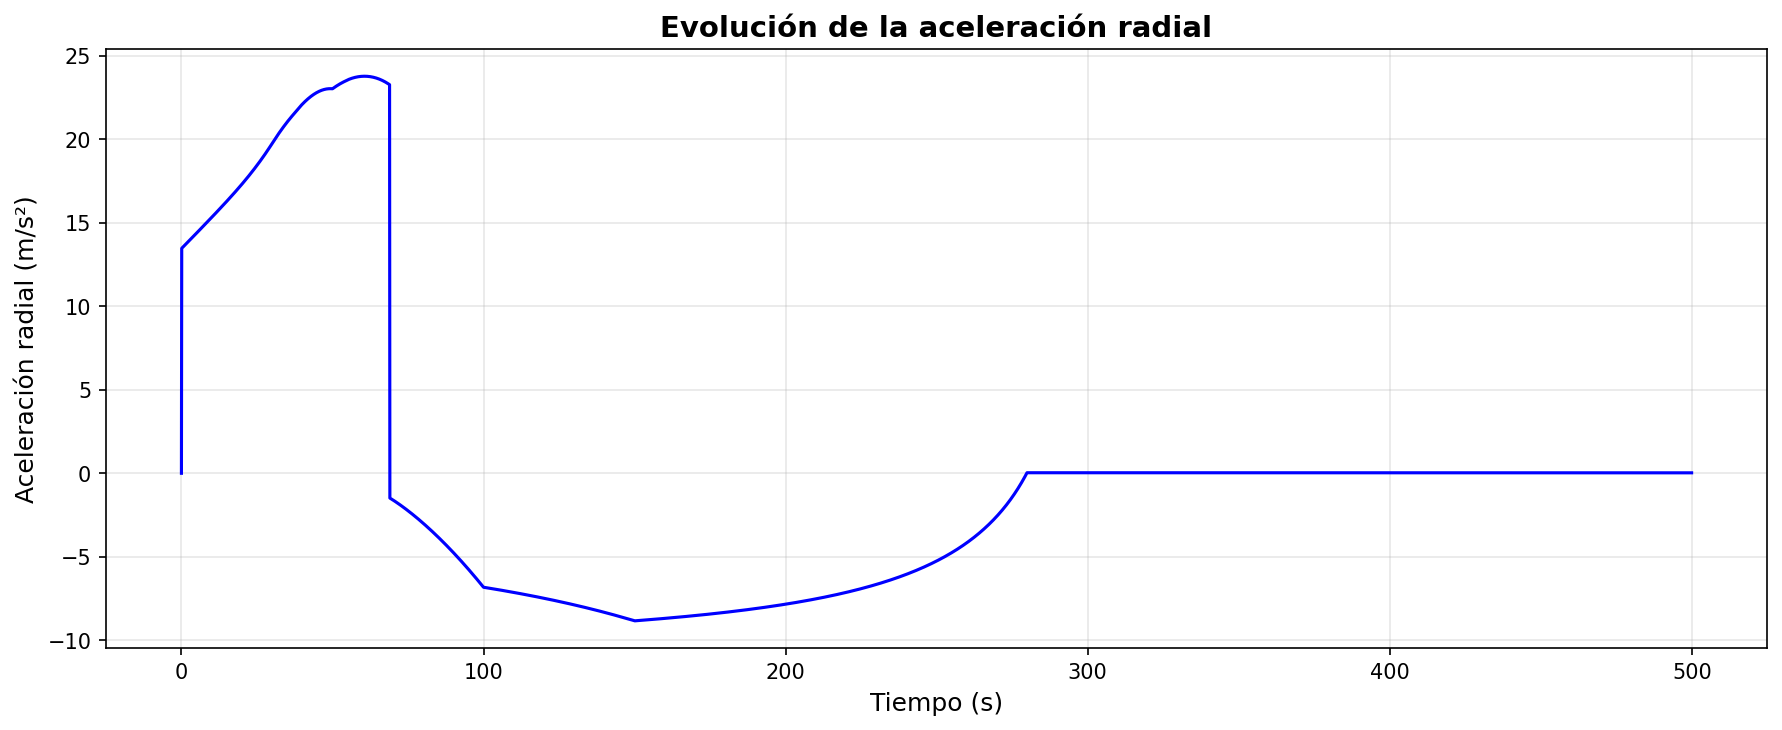
\includegraphics[width=\textwidth]{../graficos/01_aceleracion_radial.png}
    \caption{\footnotesize Acel. radial}
\end{subfigure}

\vspace{0.1cm}

\begin{subfigure}{0.32\textwidth}
    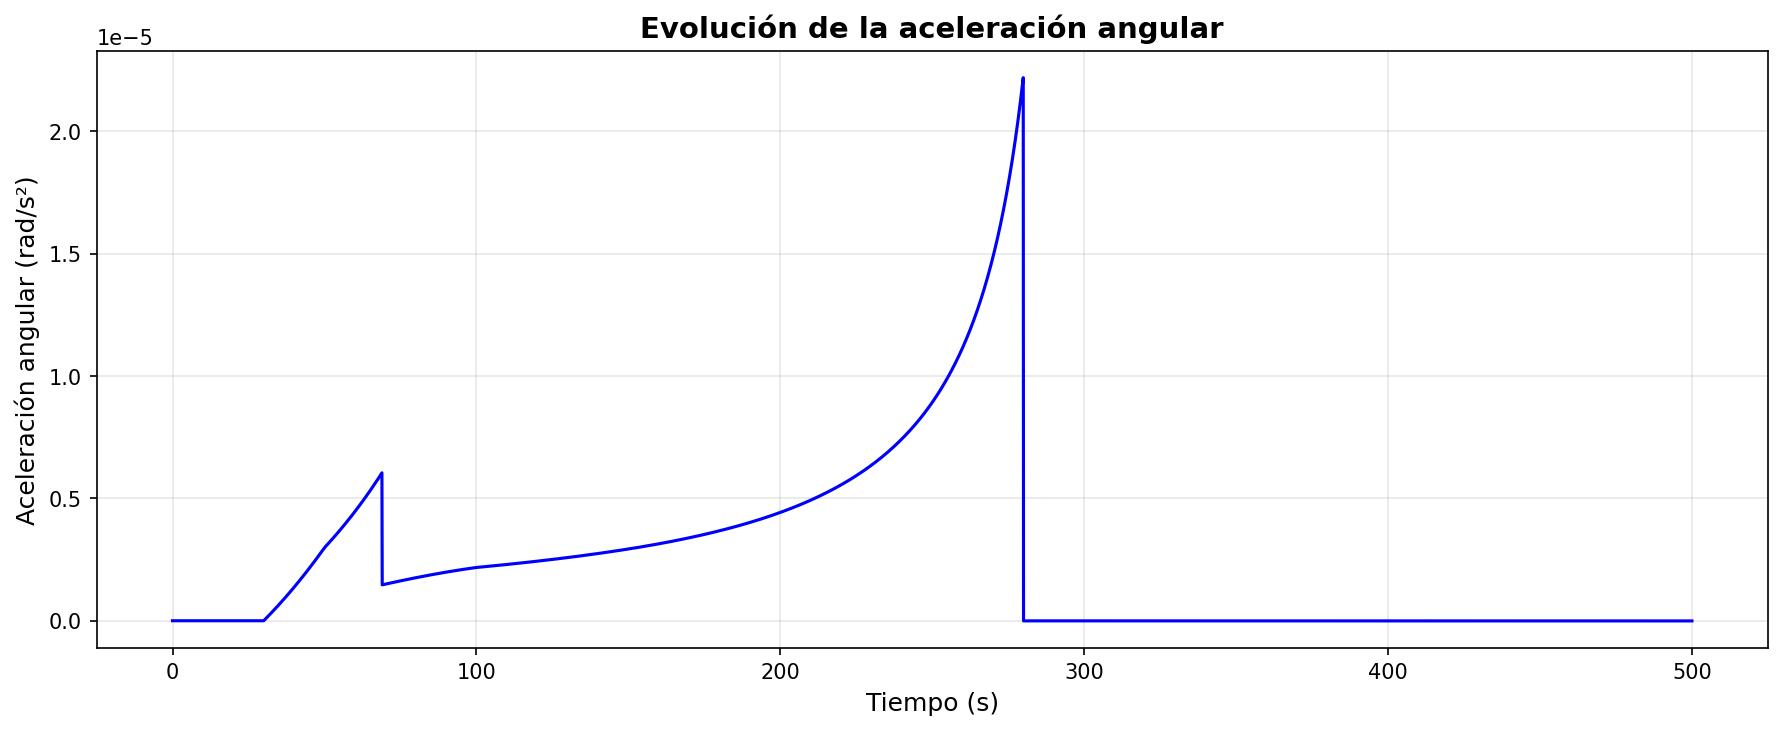
\includegraphics[width=\textwidth]{../graficos/05_aceleracion_angular.png}
    \caption{\footnotesize Acel. angular}
\end{subfigure}
\hfill
\begin{subfigure}{0.32\textwidth}
    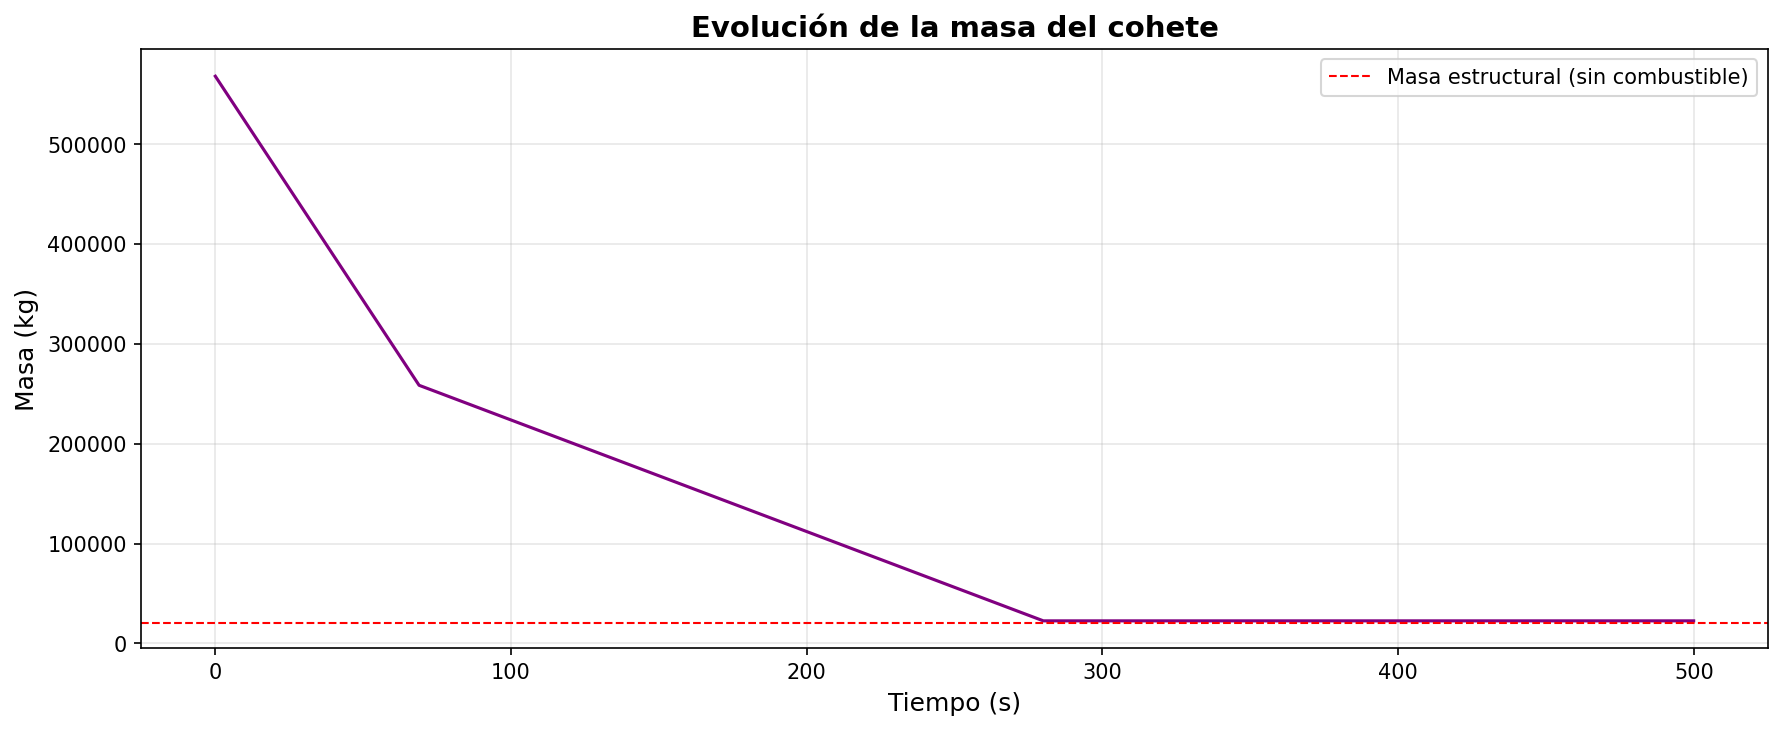
\includegraphics[width=\textwidth]{../graficos/04_masa_cohete.png}
    \caption{\footnotesize Masa}
\end{subfigure}
\hfill
\begin{subfigure}{0.32\textwidth}
    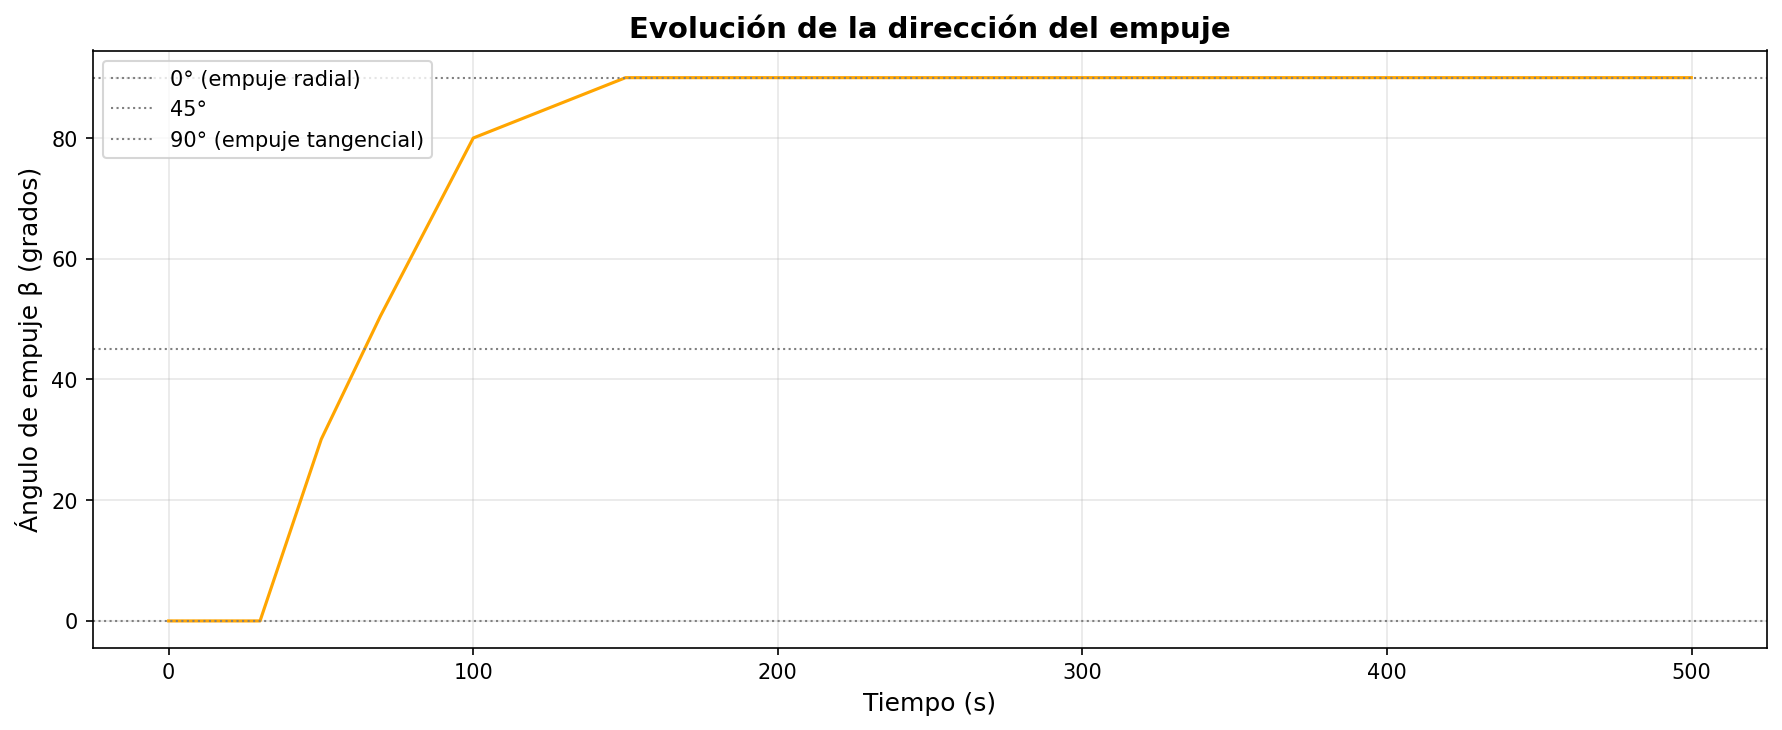
\includegraphics[width=\textwidth]{../graficos/08_direccion_empuje_beta.png}
    \caption{\footnotesize Dir. empuje}
\end{subfigure}
\caption{\small Curvas de evolución durante primeros 500s: ascenso (0-69s), circularización (69-280s), inicio órbita.}
\label{fig:curvas}
\end{figure}

% Conclusiones
\section{Conclusiones}

El simulador valida la viabilidad técnica del diseño propuesto:

\begin{itemize}
    \item \textbf{Órbita LEO lograda}: 187 km (error -6.5\%), velocidad 7,813 m/s (error +0.3\%), estable 20,000s
    \item \textbf{Perfil optimizado}: Gravity turn de dos fases minimiza pérdidas gravitatorias y aerodinámicas
    \item \textbf{Validación numérica}: Forward y Backward Euler idénticos. Tests confirman física correcta
    \item \textbf{Combustible}: 546,000 kg consumidos (99.6\% del disponible), tiempo burnout 280s. El 0.4\% restante (2,000 kg) se reserva para maniobras de emergencia y ajustes orbitales
\end{itemize}

El paso temporal $\Delta t = 0.1$s es adecuado para LEO. La desviación de 13 km es corregible ajustando momento de burnout.

\noindent\textbf{Recomendación}: Diseño listo para implementación. Cohete alcanzará órbita LEO estable con alta confiabilidad.

\end{document}